\ifx\boi\undefined\ifx\problemname\undefined
\providecommand\sampleinputname{}
\providecommand\sampleoutputname{}
\documentclass[english]{templates/boi}
\problemlanguage{.en}
\fi
\newcommand{\boi}{Baltic Olympiad in Informatics}
\newcommand{\practicesession}{Practice Session}
\newcommand{\contestdates}{April 27 - May 1, 2018}
\newcommand{\dayone}{Day 1}
\newcommand{\daytwo}{Day 2}
\newcommand{\licensingtext}{This problem is licensed under CC BY-SA 4.0.}
\newcommand{\problem}{Problem}
\newcommand{\inputsection}{Input}
\newcommand{\outputsection}{Output}
\newcommand{\interactivity}{Interactivity}
\newcommand{\grading}{Grading}
\newcommand{\scoring}{Scoring}
\newcommand{\constraints}{Constraints}
\renewcommand{\sampleinputname}{Sample Input}
\renewcommand{\sampleoutputname}{Sample Output}
\newcommand{\sampleexplanation}[1]{Explanation of Sample #1}
\newcommand{\sampleexplanations}{Explanation of Samples}
\newcommand{\timelimit}{Time Limit}
\newcommand{\memorylimit}{Memory Limit}
\newcommand{\seconds}{s}
\newcommand{\megabytes}{MB}
\newcommand{\group}{Group}
\newcommand{\points}{Points}
\newcommand{\limitsname}{Limits}
\newcommand{\additionalconstraints}{Additional Constraints}
\newcommand{\testgroups}{
Your solution will be tested on a set of test groups, each worth a number of points.
Each test group contains a set of test cases.
To get the points for a test group you need to solve all test cases in the test group.
Your final score will be the maximum score of a single submission.
}
\fi
\def\version{jury-1}
\problemname{Paths}
A {\em graph} is a mathematical structure which consists of a set of {\em vertices}, and a set of {\em edges}, each connecting two vertices. An example of a graph with $4$ vertices and $3$ edges is shown in the sample explanation below.
%For example, a road map could be a graph, if the vertices are towns or other places and the edges are roads that directly connect two places.

In this task, each vertex in the graph has one of $K$ colors. The task is to find the number of possible {\em paths} in which no two vertices have the same color. 

A {\em path} is defined as an ordered list of $2$ or more vertices, such that
there are edges between consecutive vertices in the list. Note that the list is ordered; for example, ``\texttt{1-2-3}'', ``\texttt{1-3-2}'' and ``\texttt{3-2-1}'' are all treated as different paths.


\section*{\inputsection}
The first line of input contains three integers: $N$ (the number of vertices), $M$ (the number of edges), and $K$ (the number of different colors).

%($1 \le N, M \le 3 \cdot 10^5, 1 \le K \le 5$).

The second line of input contains $N$ integers between $1$ and $K$ -- the colors of each vertex (starting with vertex $1$ and ending with vertex $N$). 

Each of the following $M$ lines describes an edge and contains two integers $a, b$ ($1 \le a, b \le N, a \neq b$) -- the two vertices connected by the edge. There will be at most one edge between any two vertices.

\section*{\outputsection}
Output one integer -- the number of paths whose vertices all have distinct colors.

\section*{\constraints}
\testgroups

\noindent
\begin{tabular}{| l | l | l |}
\hline
\group & \points & \limitsname \\ \hline
1      & 23      & $1 \le N, M \le 100, 1 \le K \le 4$ \\ \hline
2      & 20      & $1 \le N, M \le 300\,000, 1 \le K \le 3$ \\ \hline
3      & 27      & $1 \le N, M \le 300\,000, 1 \le K \le 4$ \\ \hline
4      & 30      & $1 \le N, M \le 100\,000, 1 \le K \le 5$ \\ \hline
\end{tabular}

\section*{\sampleexplanation{1}}

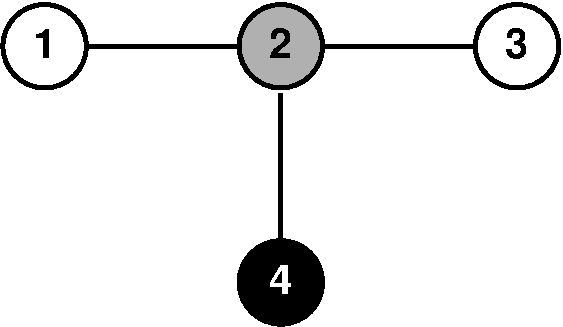
\includegraphics[width=5cm]{pathsfig.pdf}

The graph in the first example is illustrated in the figure, where each vertex has been filled with white (color 1), gray (color 2) or black (color 3). There are 10 paths whose vertices all have distinct colors: ``\texttt{1-2}'', ``\texttt{2-1}'', ``\texttt{2-3}'', ``\texttt{3-2}'', ``\texttt{2-4}'', ``\texttt{4-2}'', ``\texttt{1-2-4}'', ``\texttt{4-2-1}'', ``\texttt{3-2-4}'' and ``\texttt{4-2-3}''.

Note that ``\texttt{1}'' is not allowed as a path, because it is a single vertex, nor is ``\texttt{1-2-3}'', because it contains two nodes of color $1$.
